\chapter{The Standard Model}
\label{chap_SM}
\section{Overview}

The Standard Model (SM) describes the particles present in nature and the interactions between them. It has existed in its current form since 1974, and has been validated by numerous experiments since then~\cite{LEP,tevatron_top}. All of the particles described in the Standard Model have been observed experimentally. Most recently, the observation of a particle ``consistent'' with the Higgs boson was announced on July 4th of 2012~\cite{CernHiggsPR,ATLAS_higgs}. The cross-sections at the LHC's design specifications are shown in Figure~\ref{SMxsec} for several standard model processes. The cross-section for jet production is several orders of magnitude greater than many of the other processes of interest, and so they are produced in copius quantities at the LHC. Because of this, jets are studied extensively at \atlas, and are used to make measurements of QCD.
%
%and so measurements of jet production may be used as precise tests of QCD. \cmt{so that it can be treated as a background in other analyses.}
\begin{figure}[tb]
\begin{center}
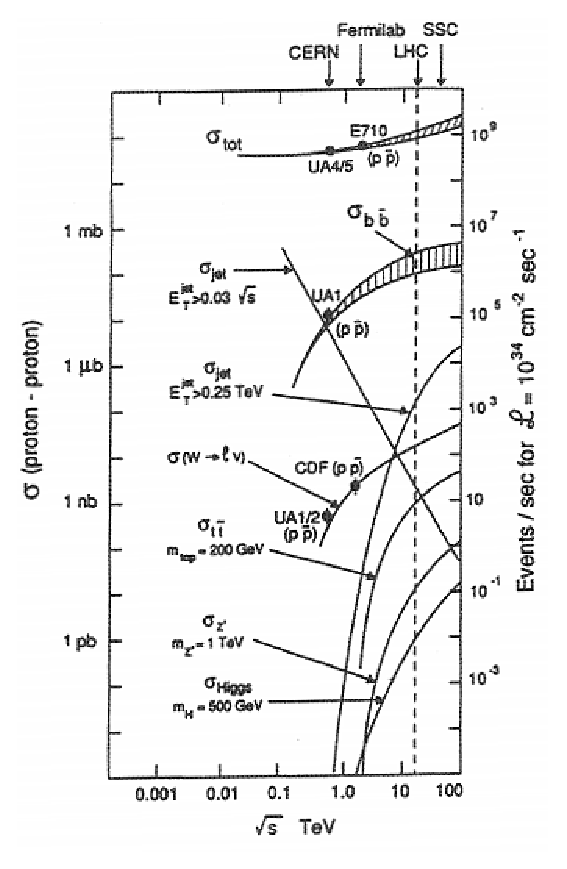
\includegraphics[width=0.4\linewidth,angle=0]{SM_xsec}
\end{center}
%\centerline{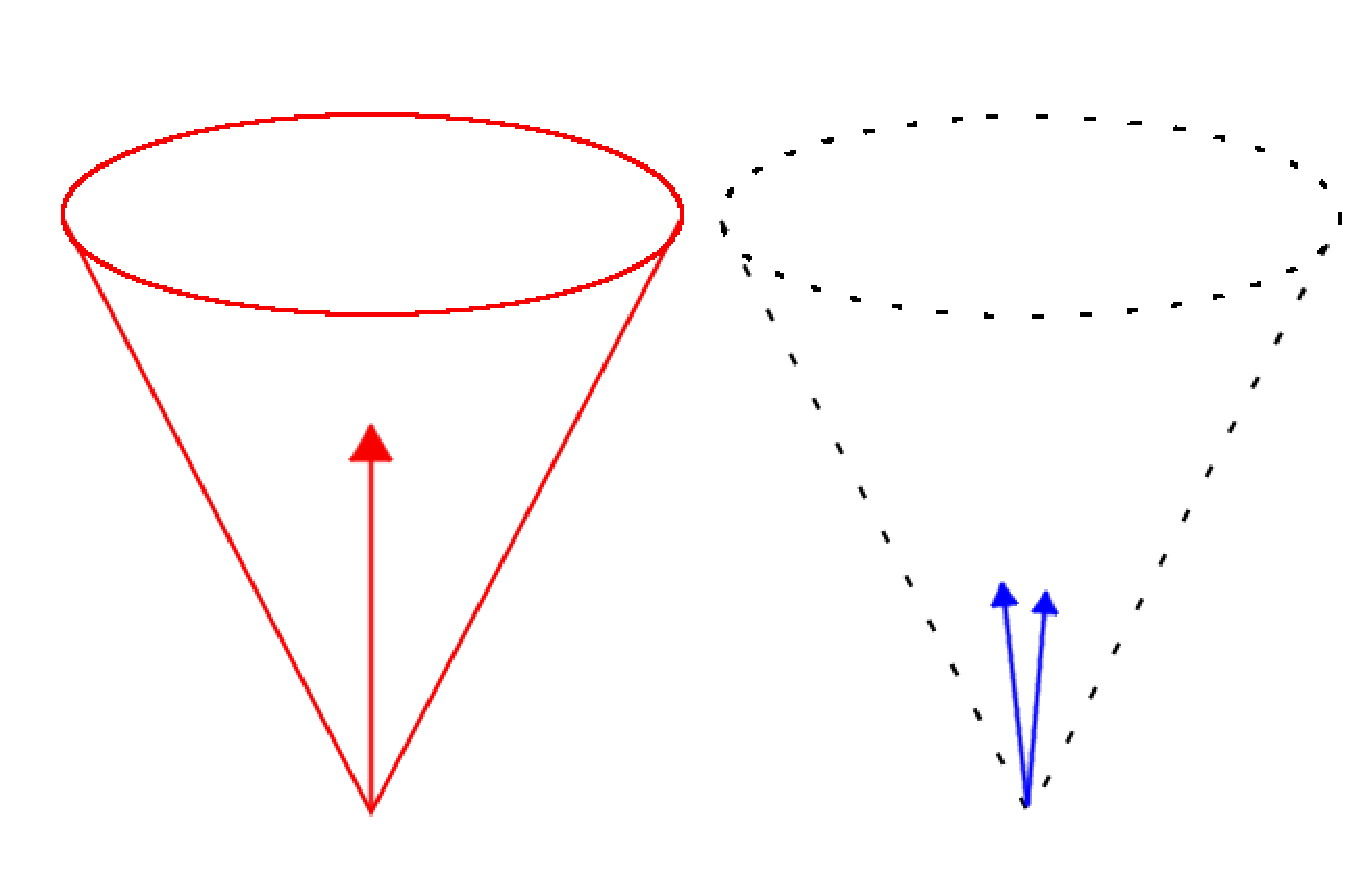
\epsfig{file=./figs/collinear.eps  , width=0.95\textwidth}}
\caption[Production cross-sections at the LHC]{Cross-sections for several SM processes as a function of the centre of mass energy of the pp collision \cite{Flugge}. The dashed line corresponds to the design energy of the LHC, while the production rates on the right are obtained using the LHC's design luminosity.}
\label{SMxsec}
\end{figure}

%At present the Higgs boson is the only Standard Model particle that hasn't yet been discovered, but ATLAS/LHC expect to have sufficient data to prove or disprove its existence by the end of 2012. 

%The fundamental building blocks of matter in the Standard Model are quarks and leptons. 

Elementary fermions in the Standard Model are divided into two groups: the quarks and leptons.  These particles represent the fundamental building blocks of matter, and there are six ``flavours'' of each. For the quarks these are the up ($u$), down ($d$), charm ($c$), strange ($s$), top ($t$), and bottom ($b$). These may be organised into generations of increasing mass, as follows,
\begin{equation}
\left( \begin{array}{c} u \\ d \end{array} \right) \quad \left( \begin{array}{c} c \\ s \end{array} \right) \quad \left( \begin{array}{c} t \\ b \end{array} \right), 
\label{SM_quark_doublets}
\end{equation}
where the upper members of each generation (the ``up type'' quarks) have electric charge +2$e$/3 and the lower members (``down type'') have charge -$e$/3, where $e$ is the absolute value of the charge on an electron. The leptons may be arranged in the same way, giving
\begin{equation}
\left( \begin{array}{c} \nu_e \\ e \end{array} \right) \quad \left( \begin{array}{c} \nu_\mu \\ \mu \end{array} \right) \quad \left( \begin{array}{c} \nu_\tau \\ \tau \end{array} \right),
\label{SM_lepton_doublets}
\end{equation}
where the lower members are the electron, muon, and tau, respectively, each having electric charge -1$e$. Each of these is paired with a neutrino ($\nu$), which is neutral and almost massless. All quarks and leptons have a spin of 1/2.\cmt{ making them fermions.}

% 
%
%
%
% The $u$, $c$, and $t$ quarks have charge $+2/3$, and are referred to as ``up-type'' quarks, while the $d$, $s$, and $b$ quarks are referred to as ``down-type'' and have charge $-1/3$. These may also be arranged into three mass generations which are, in order of increasing mass, $ud$, $cs$, and $tb$.
%
%The three charged leptons
%
% The leptons consist of the electron ($e$), the muon ($\mu$), and the tau ($\tau$), as well as their respective neutrinos: $\nu_e$, $nu_\mu$, and $nu_\tau$. 

%While the gravitational force is excluded from the Standard Model, the strong, weak and electromagnetic forces are included.


The strong, weak, and electromagnetic forces are also described by the Standard Model\footnote{Gravity is not included in the SM, but its effects are negligible at the energy scales of interest.}.
These are described by gauge theories, such that the SM Lagrangian exhibits $\su{3}_c \otimes \su{2}_L \otimes \uu{1}_Y$ symmetry. The doublets listed in equations~\ref{SM_quark_doublets} and \ref{SM_lepton_doublets} reflect the way in which the quark and lepton fields transform under the $\su{2}_L$ symmetry group, where the subscript $L$ denotes that only the left handed components of the fields take part in this interaction. The $\su{2}_L$ and $\uu{1}_Y$ symmetries together describe the electroweak sector of the Standard Model, with the subscript $Y$ referring to weak hypercharge\footnote{The weak hypercharge of a particle is the sum of its electric charge and the third component of its weak isospin ($T_3$). Up-type quarks and neutrinos have $T_3$ = 1/2, while down-type quarks and charged leptons have $T_3$ = -1/2.}.  Quantum Chromodynamics (QCD) is the gauge theory that describes the strong (or colour) force and $\su{3}_c$ is the symmetry group associated with it, where the subscript $C$ refers to colour charge.


%
%
%giving the 
%The Standard Model describes
%
% Each generation \blue{transforms} as a doublet under \su{2}, the gauge group of the weak interaction. The three generations of quarks are then
%
%%\begin{equation*}
%
%
%
%ud sc tb
%
%and for the leptons
%
%enu mu nu, tau nu
%
%The up type quarks have electric charge +2/3, while down types have charge -1/3. Electrons, mu and taus all have charge -1, while neutrinos are neutral. 
%
%
%
%
%doublets represent how fields interact via weak force.

Interactions between particles may occur via the strong force, the weak force or the electromagnetic force. All types of particles interact via the weak force, but only quarks interact via the strong force. Quarks and electrically charged leptons interact via the electromagnetic force, but neutrinos cannot.
% The Standard Model does not describe gravitational interactions between particles, however gravity is the weakest of the four forces.
All of these interactions are mediated by gauge bosons, which are excitations of the gauge fields and act as force carriers. The strong force is carried by gluons, which are massless. There are eight types of gluon, corresponding to the 8 generators of the $\su{3}_c$ symmetry associated with the strong force. There would be four massless bosons arising from the electroweak ($\su{2}_L \otimes \uu{1}_Y$) symmetry, however these symmetries are broken down to a single $\uu{1}_{EM}$ symmetry by the Higgs mechanism\cite{burgessSM}. This $\uu{1}_{EM}$ symmetry describes electromagnetic interactions, and the corresponding gauge boson is the massless photon. The other three gauge bosons associated with the broken symmetries are the $W^{+}/W^{-}$ bosons which have a mass of (80.385~$\pm$~0.015)~GeV\footnote{For simplicity, masses and momenta are listed with units of eV in this thesis, even though the eV is a unit of energy. In cases where a mass or momentum value is given in terms of eV, the unit should be understood to be eV/$\mathrm{c}^2$ or eV/c, respectively.} , and the $Z$ boson which has a mass of (91.188~$\pm$~0.002)~GeV\cite{reviewPP2012}.
% The $\su{2}_L$ and $\u{1}_Y$ sectors of the Standard Model would give rise to four massless gauge bosons,
%
%
% The gauge boson of the electromagnetic force is the photon, which is massless. The weak force has three gauge bosons:  W+/- and the Z, with masses of 82 GeV and 91 GeV respectively. The strong force is carried by gluons, which are massless. There are eight types of gluon, corresponding to the 8 generators of the SU(3) symmetry associated with the strong force.
%
%Standard Model exhibits $\su{3} \times \su{2} \times \uu{1}$ gauge symmetries. \su{3} refers to colour force, \blue{\su{2} electroweak and \uu{1} hypercharge} \red{is su2 electroweak, or is that su2 x u1?}. Interactions between particles are mediated by gauge bosons. The 8 generators of \su{3} give rise to 8 types of gluon, which mediate the colour interaction. The weak force is mediated by the W+/- and Z bosons, while the electromagnetic force is carried by the photon. The W and Z bosons have a mass of 80 and 90 GeV respectively, which they acquire when the \su{2} symmetry is spontaneously broken. a/the \uu{1} symmetry still exists \red{no - a new u1 is left over, not the same hypercharge}. after \su{2} is broken after breaking, \uu{1} becomes electromagnetism.

%In addition to the gauge bosons, the Standard Model also contains a Higgs boson.

 In addition to the weak gauge bosons, the Higgs field also allows fermionic particles to posses mass in a way that doesn't violate the gauge invariance of the SM Lagrangian. There is a potential associated with the Higgs field which causes it to spontaneously take a non-zero vacuum expectation value, breaking the electroweak symmetry mentioned earlier. Fermions interact with the Higgs field via a Yukawa coupling, and so when the Higgs field takes a vacuum expectation value these couplings act as mass terms in the Lagrangian while retaining their gauge invariance. 
  %invariance. \red{At present the Higgs boson is the only particle in the Standard Model that has not been experimentally observed. However, The \atlas experiment has narrowed the mass range of the Higgs boson to be within 115-131 GeV\cite{atlasHiggs}. If the Higgs boson exists, it is expected to be observed at \atlas by the end of 2012.}



%
%
% The \su{2} symmetry is spontaneously broken via the Higgs mechanism, which gives mass to the gauge bosons associated with the weak force. The W+/- bosons thus have a mass of 82 GeV while the Z has a mass of 90 GeV. 
%
% the $\su{2} \times \uu{1}$ symmetry is broken when Higgs takes a vev,  
%
% (this is when unified, \su{2} is electroweak and \uu{1} is hypercharge?? is this true, or is this when unified? what are the symmetries before breaking?). 
%
%Interactions between particles are mediated by gauge bosons. As the colour force exhibits \su{3} symmetry, there are eight types of gluon corresponding to the 8 generators of the \su{3} group. 
%
%should write here about how bosons relate to generators of symmetry groups. And about 
%
%
%
%
%su3 su2 u1
%colour, weak, electromagnetic
%
%quarks and leptons
%
%gauge bosons
%
%Higgs (?)
%%%%%%%%%%%%%%%%%%%%%%%%%%%%%%%%%%%%%%%%%%%%%%%%%%%%%%%%%%%%%%%%%%
%\begin{figure}[h]
%
%\centering
%\begin{fmfgraph*}(8,7)
%\fmfleft{b}
%\fmfright{c,d,ubar}
%
%\fmf{fermion, label=$b$}{b,v1}
%\fmf{fermion, label=$c$}{v1,c}
%\fmf{photon,label=$W$}{v1,v2}
%\fmf{fermion,label=$d$}{v2,d}
%\fmf{fermion,label=$\bar{u}$}{ubar,v2}
%\fmfdot{v1,v2}
%
%\end{fmfgraph*}
%\label{weak_1}
%\caption{a typical weak decay process}
%\end{figure}
%%%%%%%%%%%%%%%%%%%%%%%%%%%%%%%%%%%%%%%%%%%%%%%%%%%%%%%%%%%%%%%%%%



%quarks can form baryons: hadrons and mesons.


\section{Quantum ChromoDynamics}

%The physics of the strong force is described by Quantum ChromoDynamics (QCD), which is a non-Abelian gauge theory based on the symmetry group $\su{3}_c$. 
Quantum ChromoDynamics (QCD) is a non-Abelian gauge theory based on $\su{3}_c$. It is the strongest of the three interactions in the Standard Model, but only affects colour charged particles. As the LHC collides beams of protons, QCD is the dominant interaction. The remainder of this chapter will focus on QCD as it is the interaction responsible for jet production, which is the subject of the analysis presented in Chapter~\ref{INCJETCHAPTER}.
%As mentioned above, the gauge particles associated with QCD are gluons, of which there are 8 types.


Feynman diagrams for the three fundamental QCD vertices are shown in Figure \ref{qcd_diagram_vertices}. A major difference of QCD compared to quantum electrodynamics (QED) is that gluons carry colour charge and thus couple to one another, while the photon is uncharged. Gluon-gluon couplings can occur via the three gluon or four gluon vertices, which are depicted in Figures \ref{fig_qcd_vertex2} and \ref{fig_qcd_vertex3}. %These interactions give rise to the anti-screening effect seen in QCD, i.e. the running of the coupling constant.

%%%%%%%%%%%%%%%%%%%%%%%%%%%%%%%%%%%%%%%%%%%%%%%%%%%%%%%%%%%%%%%%%
\begin{figure}[tb]
\begin{center}
\subfigure[]{
\begin{fmfgraph*}(4,4)
\fmfleft{q1,q2}
\fmfright{g1}
\fmf{fermion}{q1,v1}
\fmf{fermion}{v1,q2}
\fmf{gluon}{v1,g1}
\fmfdot{v1}
\end{fmfgraph*}
\label{fig_qcd_vertex1}
}
\subfigure[]{
\begin{fmfgraph*}(4,4)
\fmfleft{g1,g2}
\fmfright{g3}
\fmf{gluon}{g1,v1}
\fmf{gluon}{g2,v1}
\fmf{gluon}{v1,g3}
\fmfdot{v1}
\end{fmfgraph*}
\label{fig_qcd_vertex2}
}
\subfigure[]{
\begin{fmfgraph*}(4,4)
\fmfleft{g1,g2}
\fmfright{g3,g4}
\fmf{gluon}{g1,v1}
\fmf{gluon}{g2,v1}
\fmf{gluon}{v1,g3}
\fmf{gluon}{v1,g4}
\fmfdot{v1}
\end{fmfgraph*}
\label{fig_qcd_vertex3}
}
\caption{Feynman diagrams depicting the vertices of QCD.}
\label{qcd_diagram_vertices}
\end{center}
\end{figure}
%%%%%%%%%%%%%%%%%%%%%%%%%%%%%%%%%%%%%%%%%%%%%%%%%%%%%%%%%%%%%%%%%


The coupling constant, \alphas, describes the strength of QCD interactions. This varies as a function of the transferred momentum, such that the strength of the coupling at two different momentum scales, $p^2$ and $Q^2$, are related by
\begin{equation}
%\alpha_s = \frac{4 \pi}{(11 - 2/3 N_f) \frac{-p^2}{\lqcd}  }
%\alpha_s = \frac{4 \pi}{ (11 - 2/3 N_f) \log(\frac{-p^2}{\lqcd^2})}
\alpha_s(p^2) = \frac{\alpha_s(Q^2)}{1 + \frac{11 - (2/3) N_f}{4\pi}\alpha_s(Q^2) \log (\frac{p^2}{Q^2})}
\label{eqn_alpha_s_1}
\end{equation}
%
%where $q^2$ and $Q^2$ are the...
where $N_f$ is the number of quark flavours with mass less than $p^2$.
The ``QCD scale'', \lqcd, is defined as the scale at which the denominator of equation~\ref{eqn_alpha_s_1} vanishes, i.e.
\begin{equation}
\frac{11 - (2/3) N_f}{4\pi} \, \alpha_s(Q^2) \,\log (\frac{\lqcd^2}{Q^2}) = -1.
\end{equation}
Using this definition, equation~\ref{eqn_alpha_s_1} becomes
\begin{equation}
%\alpha_s = \frac{4 \pi}{(11 - 2/3 N_f) \frac{-q^2}{\lqcd}  }
%\alpha_s = \frac{4 \pi}{ (11 - 2/3 N_f) \log(\frac{-q^2}{\lqcd^2})}
\alpha_s(p^2) = \frac{4 \pi}{(11 - (2/3) N_f) \log (\frac{-p^2}{\lqcd^2})}.
\label{eqn_alpha_s_3}
\end{equation}


%some values of $\alpha_s$. 
The value of \lqcd~is around 200-300 MeV. This does not mean that the coupling constant is infinite at \lqcd, merely that the perturbative calculations used in the derivation of equation~\ref{eqn_alpha_s_1} are no longer valid in this regime. When measured at the mass of the $Z$ boson,  $\alphas (M_Z) =0.1184$~\cite{reviewPP2012}, indicating that perturbation theory is reliable at this energy scale. 
%%%%%%%%%%%%%%%%%%%%%%%%%%%%%%%%%%%%%%%%%%%%%%%%%%%%%%%%%%%%%%%%%
\begin{figure}[h]
\begin{center}
\subfigure[]{
\begin{fmfgraph*}(3,3)
\fmfleft{q1,q2}
\fmfright{q3,q4}
\fmf{fermion}{q1,v1}
\fmf{fermion}{v1,q2}
\fmf{fermion}{q3,v2}
\fmf{fermion}{v2,q4}
\fmf{gluon}{v1,v2}
\fmfdot{v1}
\fmfdot{v2}
\end{fmfgraph*}
\label{fig_qcd_tree}
}
\subfigure[]{
\begin{fmfgraph*}(3,3)
\fmfleft{g1}
\fmfright{g2}
\fmf{gluon, tension=2}{g1,v1}
\fmf{gluon, tension=2}{g2,v2}
\fmf{fermion, left, tension=0.4}{v1,v2,v1}
\fmfdot{v1}
\fmfdot{v2}
\end{fmfgraph*}
\label{fig_qcd_NLOq}
}
\subfigure[]{
\begin{fmfgraph*}(3,3)
\fmfleft{g1}
\fmfright{g2}
\fmf{gluon, tension=2}{g1,v1}
\fmf{gluon, tension=2}{g2,v2}
\fmf{gluon, left, tension=0.4}{v1,v2,v1}
\fmfdot{v1}
\fmfdot{v2}
\end{fmfgraph*}
\label{fig_qcd_NLOg3}
}
\subfigure[]{
\begin{fmfgraph*}(3,3)
\fmfleft{g1}
\fmfright{g2}
\fmf{gluon, tension=2}{g1,v1}
\fmf{gluon, tension=2}{g2,v1}
\fmf{gluon, left, tension=0.8}{v1,v1}
\fmfdot{v1}
\end{fmfgraph*}
\label{fig_qcd_NLOg4}
}

\caption[Tree level $qq\rightarrow qq$ scattering]{Tree level $qq\rightarrow  qq$ scattering, and vacuum polarisation diagrams. }
\label{qcd_LO_NLO}
\end{center}
\end{figure}
%%%%%%%%%%%%%%%%%%%%%%%%%%%%%%%%%%%%%%%%%%%%%%%%%%%%%%%%%%%%%%%%%

A leading order diagram for a $qq \rightarrow qq$ process is shown in Figure \ref{fig_qcd_tree}, where four-momentum is exchanged between two quarks via a gluon. At next to leading order (NLO), the gluon propagator in Figure \ref{fig_qcd_tree} may be replaced by the vacuum polarisation diagrams shown in Figures \ref{fig_qcd_NLOq}-\ref{fig_qcd_NLOg4}. The first of these diagrams, Figure~\ref{fig_qcd_NLOq}, causes the vacuum to effectively screen colour charge, such that at large distances the strength of the interaction is diminished. A similar effect occurs in Quantum ElectroDynamics (QED), the quantum field theory describing the electromagnetic interaction. A diagram analogous to Figure~\ref{fig_qcd_NLOq} exists in QED, which gives rise to the running of the electromagnetic coupling constant.%This is what happens in QED, and is the reason why the effective coupling constant $\alpha_{\mathrm{QED}}$ decreases at  higher momenta. 

The three and four gluon vertices in Figure~\ref{qcd_diagram_vertices} give rise to the diagrams in Figures \ref{fig_qcd_NLOg3} and \ref{fig_qcd_NLOg4}. The gluon loops in these diagrams cause an anti-screening effect, such that the strength of the interaction decreases as the exchanged four-momentum increases. This is the opposite effect to that seen for the quark loop, however in QCD it is this effect that dominates. 



%The value of \lqcd~is around 200-300 MeV, while the strong coupling measured at the $Z$ bosons mass, $m_Z$, is $\alphas (MZ) =0.12$. Doesn't mean that the coupling is infinite at, \lqcd, merely that the perturbative calculations used in the derivation of equation~\ref{eqn_alpha_s_1} are no longer valid in this regime.

%where $q^2$ is the transferred momentum and $Q^2$ is the scale at which the theory is renormalised.
%\red{change this. Describe alpha(Q2) as a function of Q02. Then define lambdaqcd}
% lambda QCD.


The anti-screening effect is characteristic of \su{N} gauge theories. An \su{4} theory would contain four colours and 15 gluon fields ($N^2 -1$), increasing the contribution of the gluon loop diagrams in Figure~\ref{qcd_LO_NLO} and thus increasing the anti-screening effect. Conversely, a QCD-like theory based on \su{2} would contain 3 gluons (like the three gauge bosons of the weak force), which would result in a smaller anti-screening effect. The screening effect, however, increases with the number of quark fields contained in the theory. For example, in \su{3} gauge theories that contain 17 or more quark flavours the screening effect is dominant and the strength of the interaction increases as the exchanged four-momentum increases, as can be seen from equation~\ref{eqn_alpha_s_3}.\cmt{ ~\cite{greiner2007quantum}. }



\subsection{Factorisation}
\label{sec_factorisation}
%\red{maybe put stuff on pp collisions here}

%QCD lets us do parton parton scattering, perturbative, easy.
%
%computing results of a proton proton collision difficult, because while the momentum scale is good for perturbation theory, physics related to the structure of the proton determined at \lqcd, so there are two different scales to the problem. 

%Factorisation allows physics at these scales to be separated. Low momentum, non-perturbative physics describing the structure of the proton can be isolated from the high momentum, perturbative physics of the parton-parton scattering.
%
%like perturbation theory. At high momenta, this is what we have, and things may be described in terms of quarks and gluons. At low momenta, non perturbative. Proton-proton scattering is then difficult, as the proton must be described non-perturbatively. Difficult to obtain theoretical model of a proton.
%
%problem arises because two different scales are involved in the problem. structure of the proton determined by effects at \lqcd, while the scale relevant for the scattering is dependant on the exchanged momenta, $q^2$, which is at the TeV scale for collisions at the LHC.
%
%factorisation allows proton scattering to be separated into momentum dependent parts calculable via perturbation theory, and non-perturbative, momentum independent parts that describe the structure of the proton.



%can factorise things. Can't use perturbation theory to understand structure of the proton, however this can be expressed in terms of Parton Distribution Functions. 

%Fortunately, things may be factorised\red{cite factorisation}. Deep inelastic scattering.
%
%\red{cite burgess, look for masters report also, there were some things about factorisation in there also} Know what the electromagnetic parts look like, know what form the hadronic current has to take. Can thus express the proton in terms of structure functions, describe the structure of the proton. These describe the non-perturbative effects. Can't calculate them using perturbation theory, but can use lattice QCD models, or measure them from experiment.
%
%Structure functions, in turn, may be expressed in terms of parton distribution functions (PDFs).
 
 
Theoretical descriptions of proton-proton collisions are complicated, as different energy scales are involved in the problem. The four-momentum exchanged between partons can be at the TeV scale for collisions at the LHC, while the physics describing the arrangement of the partons within the proton is determined at a much lower scale, \lqcd. QCD is a strongly coupled theory at low energies, whereas at higher energies it is weakly coupled and perturbative methods may be used. Fortunately, factorisation  allows the physics at these different scales to be separated~\cite{Collins1985104}. The low-momentum, non-perturbative physics describing the structure of the proton may be isolated from the high momentum, parton-parton scattering. 
 
 The structure of the proton may thus be described using Parton Distribution Functions (PDFs), $q_i(x,Q^2)$, $G(x,Q^2)$, and $\overline{q}_i(x,Q^2)$. The functions $q_i(x,Q^2)$ describe the probability of a probe (such as an electron or parton) with momentum $Q^2$ finding a quark of flavour $i$ within the proton, with said quark carrying a fraction $x$ of the proton's momentum\cite{burgessSM}. Similarly, the distribution functions $\overline{q_i}(x,Q^2)$ and $G(x,Q^2)$ describe the probability of finding an anti-quark or gluon, respectively, within the proton. While a proton is typically thought of as containing two up quarks and one down quark, it also contains gluons, which together carry about half of the proton's momentum~\cite{burgessSM}. Gluons may also split into quark-antiquark pairs, referred to as ``sea'' quarks. Because of this, the probabilities of finding antiquarks (or quarks with flavours other than up or down) are non-zero, and vary as a function of $Q^2$\cite{greiner2007quantum}. The number of valence quarks is conserved, however, giving the conditions
\begin{eqnarray}
\int_0^1 dx \left[q_{\mathrm{up}} (x,Q^2) - \overline{q}_{\mathrm{up}}(x,Q^2)\right] & = & 2 \\
\int_0^1 dx \left[q_{\mathrm{down}} (x,Q^2) - \overline{q}_{\mathrm{down}}\}(x,Q^2)\right] & = & 1 \\
\int_0^1 dx \left[q_{j} (x,Q^2) - \overline{q}_{j}(x,Q^2)\right] & = & 0 \quad,\quad j \in \{c,s,t,b\}
\end{eqnarray}

%\red{other conditions}
%\red{equation for cross-section expressed in terms of PDFs}



While the parton distribution functions must be determined from experiment, their $Q^2$ dependence can be calculated in a similar fashion to that of the coupling constant, \alphas. The dependence of the PDFs on $Q^2$ is given by the Dokshitzer - Gribov - Lipatov - Altarelli - Parisi (DGLAP) equations~\cite{burgessSM,Altarelli1977298}:

\begin{eqnarray}
\frac{ \ud q_i (x, Q^2)}{\ud \log Q^2} & = & \frac{ \alphas}{2 \pi } \int_x^1 \frac{\ud y}{y}\left[ P_{qq}(y)q_i(\frac{x}{y},Q^2) + P_{qG}(y)G(\frac{x}{y},Q^2) \right] \\
\frac{\ud \overline{q_i}(x,Q^2)}{\ud \log Q^2} & = & \frac{\alphas}{2 \pi} \int_x^1 \frac{\ud y}{y}\left[ P_{qq}(y)\overline{q_i}(\frac{x}{y},Q^2) + P_{qG}(y)G(\frac{x}{y},Q^2) \right] \\
\frac{\ud G(x,Q^2)}{\ud \log Q^2} & = & \frac{\alphas}{2 \pi} \int_x^1 \frac{\ud y}{y}\left[ P_{Gq}(y) \sum_i \left(q_i(\frac{x}{y},Q^2) + \overline{q_i}(\frac{x}{y},Q^2) \right) \right. \nonumber\\ & & \left.+ P_{GG}(y)G(\frac{x}{y},Q^2) \right], 
\label{eqn_DGLAP}
\end{eqnarray}
where the $P_{xx}$ are splitting functions. While a probe at $Q^2$ may see a quark or gluon within the proton, a probe with higher momentum may be able to resolve finer structures that are only present for a short time. For example, a given probe may be able to resolve a quark, while a probe with higher momentum may be able to interact with a collinear gluon emitted by this quark (Figure~\ref{fig_Pqq}). Similarly, a high momentum probe may be able to resolve a quark or antiquark (Figure~\ref{fig_PqG}), or another gluon (Figure~\ref{fig_PGG}), which are produced by a gluon. The splitting function $P_{Gq}(y)$ describes the probability for a quark to emit a colinear gluon, with the gluon carrying a fraction $y$ of the quark's momentum. The complementary function $P_{qq}(y)$ describes the probability that the quark will retain a fraction $y$ of its momentum after this emission. The function $P_{qG}(y)$ describes the probability for a gluon to split into a quark/anti-quark pair, with one of the products carrying a fraction $y$ of the gluon's momentum, while $P_{GG}(y)$ is the probability for a gluon to emit another gluon that carrys a fraction $y$ of its momentum. 


% These allow measurement of the PDFs to be made independently of probe momentum. 


%%%%%%%%%%%%%%%%%%%%%%%%%%%%%%%%%%%%%%%%%%%%%%%%%%%%%%%%%%%%%%%%%
\begin{figure}[h]
\begin{center}
\subfigure[]{
\begin{fmfgraph*}(3,3)
\fmfleft{q1,qfake,q3}
\fmftop{g3}
\fmf{fermion}{q1,v1}
\fmf{fermion}{v1,q3}
\fmf{gluon, tension=0.2}{v1,g3}
\fmfdot{v1}
\end{fmfgraph*}
\label{fig_Pqq}
}
\subfigure[]{
\begin{fmfgraph*}(3,3)
\fmfbottom{g1}
\fmftop{q2,q3}
\fmf{gluon, tension=40}{g1,v1}
\fmf{fermion,right=0.5, tension=15}{v1,q3}
\fmf{fermion,right=0.5, tension=15}{q2,v1}
%
%\fmf{fermion, tension=10}{i1,q3}
%\fmf{fermion, tension=10}{q2,i2}
\fmfdot{v1}
\end{fmfgraph*}
\label{fig_PqG}
}
\subfigure[]{
\begin{fmfgraph*}(3,3)
\fmfleft{q1,qfake,q3}
\fmftop{g3}
\fmf{gluon}{q1,v1}
\fmf{gluon}{v1,q3}
\fmf{gluon, tension=0.2}{v1,g3}
\fmfdot{v1}
\end{fmfgraph*}
\label{fig_PGG}
}



\caption[Processes described by splitting functions]{Processes described by the splitting functions. In (a), a colinear gluon is emitted by a quark, while in (b) a gluon splits into a quark antiquark pair. In (c), a gluon emits another gluon.}
\label{qcd_splitting_functions}
\end{center}
\end{figure}
%%%%%%%%%%%%%%%%%%%%%%%%%%%%%%%%%%%%%%%%%%%%%%%%%%%%%%%%%%%%%%%%%

%\blue{While the non-perturbative structure of the proton cannot be derived analytically from QCD, this structure may be represented in terms of the parton distribution functions. The evolution of the PDFs with respect to the probe momenta may be derived, which allows the PDFs to be determined from experimental measurements}. 
The PDFs derived by the CT10 group~\cite{CT10_note} are plotted in Figure \ref{CT10_fig}, for $Q^2 = $ 1 TeV. These are derived from a global analysis of data collected from many experiments. Most recently, the results of fixed target deep inelastic scattering experiments carried out at HERA~\cite{Hera}, as well as data obtained from proton-proton collisions at the Tevatron~\cite{Tevatron}, have been included in the CT10 analysis. At small $x$ the gluon PDF is dominant, and consequently the sea quark contributions are also significant in this regime, whereas the valence quarks dominate at higher values of $x$.
%%%%%%%%%%%%%%%%%%%%%%%%%%%%%%%%%%%%%%%%%%%%%%%%%%%%%%%%%%%%%%%%%
\begin{figure}[h]
\begin{center}
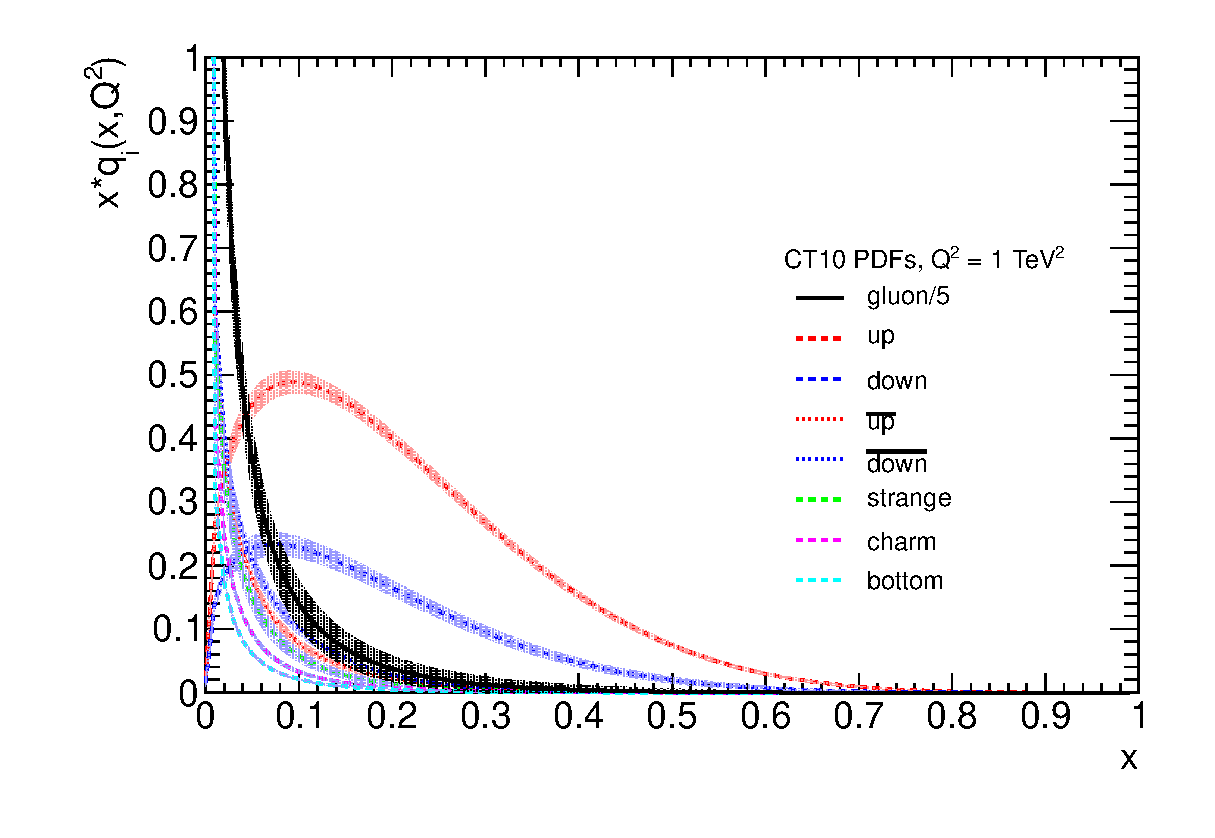
\includegraphics[width=0.8\linewidth,angle=0]{CT10_1TeV_errs.eps}
\end{center}
%\centerline{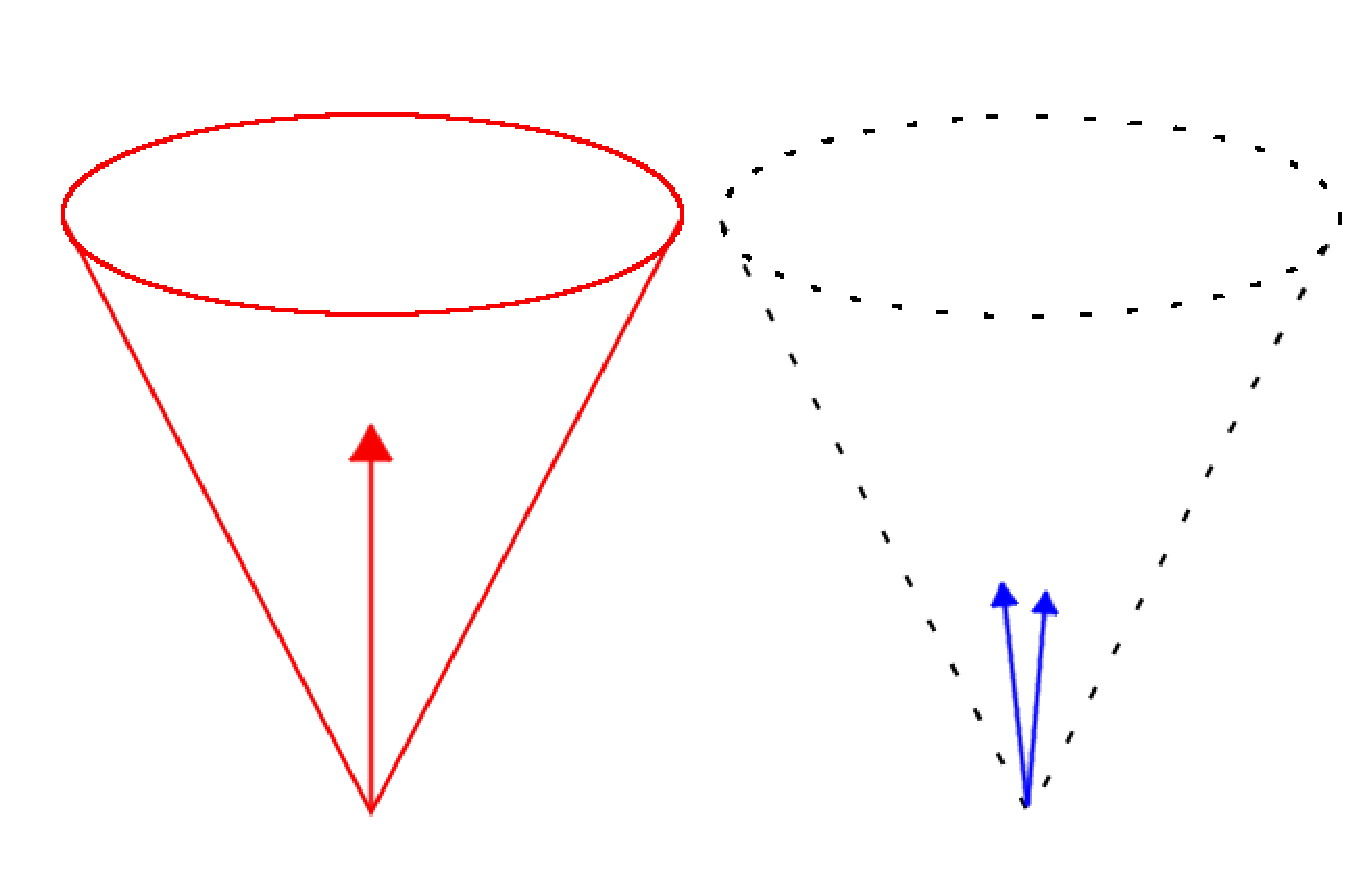
\epsfig{file=./figs/collinear.eps  , width=0.95\textwidth}}
\caption[CT10 parton distribution functions]{CT10 PDFs, obtained at a $Q^2$ scale of 1 TeV~\cite{CT10_note,hepdata}. Note that the $y$ axis shows the product of the PDF and $x$. The area under a given curve thus corresponds to the relative amount of the proton's momentum carried that type of parton. The up and down quark curves show the valence quark contributions only: the contributions from sea quarks are equal to the antiquark curves.}
\label{CT10_fig}
\end{figure}
%%%%%%%%%%%%%%%%%%%%%%%%%%%%%%%%%%%%%%%%%%%%%%%%%%%%%%%%%%%%%%%%%


\subsection{Perturbative QCD}

%Have some pdfs now, so the cross-section for a given process may be written as

The cross-section for producing a final state, $X$, from two protons with four-momentum $p_A$ and $p_B$ may be written as~\cite{hard_quarks}
\begin{equation}
\sigma_{pp \rightarrow X} =   \sum_{i,j}\int_0^1 \ud x_1 \,\int_0^1 \ud x_2 \, f_{i,A}(x_1,Q^2)\, f_{j,B} (x_2,Q^2)\, \hat{\sigma}_{i,j \rightarrow X}(x_1 p_A\, , x_2 p_B),
\end{equation}
where $f_{i,A}$ is the parton distribution function describing the probability of finding a parton of flavour $i$ within proton $A$, and the sum runs over all parton types. The partonic cross-section, $\hat{\sigma}_{i,j \rightarrow X}$ , describes the probability of producing the final state $X$ from the incoming partons of flavour $i$ and $j$, and may be calculated order by order in perturbation theory.

A leading order (LO) diagram for a $2\rightarrow 2$ process is shown in Figure~\ref{fig_pqcd_tree}. Leading order contributions are the easiest to calculate, but are generally only correct to within an order of magnitude for QCD processes~\cite{CataniSeymour}. Theoretical predictions that are to be compared with experimental measurements usually need to be made at next-to-leading order (NLO) or higher.

At NLO, virtual corrections arising from loop diagrams (such as the one shown in Figure~\ref{fig_pqcd_NLOq}) must  be considered. These virtual corrections contain ultraviolet divergences, which may be removed through renormalisation. However, there are also infrared divergences present, such that the result diverges in cases where the energy of an incoming or outgoing parton vanishes (``soft'' divergence), or in cases where the separation between two of the initial or final state partons vanishes (a ``collinear'' divergence). These infrared divergences cannot be removed, and so any calculation carried out to a fixed order in perturbation theory that considers a specific number of partons in the final state will diverge~\cite{new_method}. In order to obtain a physical result at fixed order in perturbation theory, real corrections must be considered. These real corrections include cases where an additional parton is emitted by one of the incoming or outgoing partons, such as that shown in Figure~\ref{fig_pqcd_NLOg3}. The real corrections also include collinear and soft divergences, but of the opposite sign to those present in the virtual corrections. In fixed order calculations in which both real and virtual contributions are considered, the infrared divergences cancel to give a finite result\cite{CataniSeymour}. 
%%%%%%%%%%%%%%%%%%%%%%%%%%%%%%%%%%%%%%%%%%%%%%%%%%%%%%%%%%%%%%%%%
\begin{figure}[tb]
\begin{center}
\subfigure[]{
\begin{fmfgraph*}(4,4)
\fmfleft{q1,q2}
\fmfright{q3,q4}
\fmf{fermion}{q1,v1}
\fmf{fermion}{v1,q2}
\fmf{fermion}{q3,v2}
\fmf{fermion}{v2,q4}
\fmf{gluon}{v1,v2}
\fmfdot{v1}
\fmfdot{v2}
\end{fmfgraph*}
\label{fig_pqcd_tree}
}
\subfigure[]{
\begin{fmfgraph*}(4,4)
\fmfleft{q1,q2}
\fmfright{q3,q4}
\fmf{gluon}{v1,v2}
\fmf{gluon}{v3,v4}
\fmfdot{v1,v2,v3,v4}
\fmf{fermion,left,tension=0.5}{v2,v3,v2}
\fmf{fermion}{q1,v1,q2}
\fmf{fermion}{q3,v4,q4}
\end{fmfgraph*}
\label{fig_pqcd_NLOq}
}
\subfigure[]{
\begin{fmfgraph*}(4,4)
\fmfleft{q1,q2}
\fmfright{q3,g3,q4}
%\fmf{gluon}{v1,v2}
%\fmf{fermion,left, tension=2}{q1,v1,q2}
%\fmf{fermion,left, tension=2}{v2,v3}
%\fmf{gluon, right, tension=5}{v3,g3}
%\fmf{fermion,left, tension=5}{q4,v2}
%\fmf{fermion,right, tension=5}{q3,v3}
\fmf{gluon}{v1,v2}
\fmf{fermion}{q1,v1,q2}
\fmf{fermion}{q3,v2,v3,q4}
\fmffreeze
\fmf{gluon}{v3,g3}
\fmfdot{v1}
\fmfdot{v2}
\fmfdot{v3}
\end{fmfgraph*}
\label{fig_pqcd_NLOg3}
}
\caption[Diagrams for $qq \rightarrow qq$ scattering]{Diagrams for $qq \rightarrow qq$ scattering. The tree diagram in (a) contributes at leading order, while the virtual correction in (b) and the real correction in (c) contribute at NLO.}
\label{pqcd_LO_NLO}
\end{center}
\end{figure}


\subsection{Soft Processes in Proton-Proton Collisions}


%When analysing proton-proton collisions, the most interesting

The products of hard scatterings between partons are usually considered the most interesting parts of proton-proton collisions. However, there are other important processes involved in these collisions. Partons entering or leaving the hard scattering may undergo bremsstrahlung emission, producing initial (or final) state radiation. 

There are also underlying event (UE) effects associated with the proton remnants, i.e. other partons that were constituents of the initial protons but were not involved in the hard scattering. These partons may undergo soft scatterings amongst themselves (multiple parton interactions), and may also radiate before/after these interactions.

``Pile-up'' is another issue affecting the LHC\footnote{While pileup is a significant issue at the LHC's design luminosity (and at present), it was not a major concern during 2010. At the end of the 2010 data-taking period, there were $\sim$ 3.5 collisions occuring during each bunch crossing}.  The LHC collides bunches containing $\sim 10^{11}$ protons. At the LHC's design specifications, it is rare for only a single scattering to occur during bunch crossings, with (on average) $\sim23$ collisions occuring between different pairs of protons every bunch crossing. The majority of these collisions are soft, producing low \pt~products. However, the energy deposited in the calorimeter by pile-up needs to be accounted for when measuring other high \pt~objects, particularly jets.
%\blue{biggest obstacle with ??}
%\red{MORE about pileup/minbias here}

%%%%%%%%%%%%%%%%%%%%%%%%%%%%%%%%%%%%%%%%%%%%%%%%%%%%%%%%%%%%%%%%%
\subsection{Hadronisation and Jet Production}

%Any partons produced in a collision will continue to interact via the colour force. However, the strength of the coupling increases approximately linearly with the separation between these partons. \red{DO SOMETHING ABOUT THIS}This increases the probability that an initial parton will collinearly radiate other partons, in a process referred to as showering. While there may initially be only a few partons produced by the hard scattering, those partons will multiply, with each evolving into a collimated shower of partons.

%\red{cite something about confinement and string tension}
%These partons will then arrange themselves into hadrons. 
After the hard scattering and emission of any final state radiation, partons will continue to interact via the colour force. As the separation between these partons increases, the strength of the interaction also increases. 

The confinement hypothesis states that colour charged partons do not exist in isolation; they must be confined within colourless hadrons\cite{burgessSM}. All hadrons observed in nature consist of quarks and gluons arranged in colour singlet (i.e. colour neutral) states. If a given quark were to be separated from the other constituents in its parent hadron in order to ``isolate'' it, the energy required to achieve this would increase with the separation distance. At a certain point it becomes energetically favourable for a quark-antiquark pair to be produced from the vacuum, such that the remnants of the parent hadron form a bound state with one member of the new pair, while the separated quark binds with the other member of the pair. It is thus not possible to observe a free quark in isolation, as new hadrons are formed instead using partons created from the vacuum. 

Partons emerging from the collision thus organise themselves into collimated sprays of hadrons, which are referred to as ``jets''. The showering and hadronisation of particles are non-perturbative processes, and so it is difficult to predict the way in which a parton produced in a collision will evolve into a jet. Jets will be discussed further in chapter~\ref{INCJETCHAPTER}, which describes the experimental measurement of the inclusive jet cross-section. 

%
%
%QCD and collider physics /   R.K. Ellis, W.J. Stirling, B.R. Webber.
%QC793.3 .Q35 E44 1996X, gerstein
%
%
%
%
%need to talk about pp collisions,  isr, fsr, underlying event, pileup, etc. in this subsection.
%Theoretical calculations may be made using perturbation theory \red{mention alphas, it's small, go order by order in powers of alphas}. 
%
%
%However, Leading order results are somewhat crude, and really only correct to within an order of magnitude. Not suitable for comparison with precise measurements. 
%
%pp collisions contain physics at different scales
%long distance physics describes isr/fsr, underlying event, parton showering and hadronisation
%
%short distance physics high momentum hard scattering, done via pqcd.
%
%maybe move above section down to here.
%maybe start "PP" section at factorisation.
%
%OR
%just talk about other things, UE, isr/fsr here. Then next subsection can be pqcd, then section on event generators.
%







%\section{perturbative QCD and Monte Carlo Event Generators}






%This makes calculations at NLO complicated. 


\subsection{Monte Carlo Event Generators}

%would like to make some theoretical predictions.
%
%have pdfs
%
%theory is complicated though, especially going beyond leading order (tree level). for a pp->2 jets process, things are ok at LO. at NLO, need to consider loop corrected 2->2 processes (like with running alphas) as well as 2->3 processes involving collinear or soft radiation. 
%
%pp collision has three parts, ISR, hard scatter, FSR.  pdfs + perturbation theory can do the hard scatter no problem.
%
%isr and fsr are tricky though
%
%two approaches. shower monte carlos calculate the hard scatter, and then use showering models to develop any fsr from the products of the scatter. isr is handled in reverse: the partons involved in the hard scattering are built back up, showered in reverse.
%
%
%
%
%
%SMCs - do hard scatter at tree level/LO. then shower products/incoming partons - this is the NLO part
%
%like NLO - but the whole process is not at NLO accuracy
%
%SMCs are not accurate enough to directly compare to measured data. use SMCs to correct data for detector effects, then compare unfolded data to NLO (actual NLO) predictions
%
%would like SMCs to be NLO, but this is tricky. some things are at NLO in the showering part, but not in the hard scattering part. if the hard scatter were just done to NLO, then there be some NLO corrections counted twice, things wouldn't be consistent.
%
%SMCs work to leading logs (LL). part of this is at NLO.
%
%
%so pythia is LO at hard scatter(matrix element?), parton showering is leading log. 
%
%powheg is NLO. hard scatter is done NLO, with LL part of parton showering subtracted. Then parton showering is applied, result is NLO. can be interfaced to SMCs. 
%
%how does NLOJET++ work - uses catani-seymour method. I think \powheg uses the same method, or similar?
%
%
%how do SMCs (pythia, Herwig) work?
%
%ALPGEN? may be mention in JES stuff.
%
%
%%read MC\_generators_611247.pdf
%
%
%
%
%MC event generators.
%
%tree level calculations easy.
%
%NLO: has loop graphs, + diagrams that emit gluon radiation. ISr/FSR
%
%shower MC: pythia/Herwig: do the matrix element, 2->2 at tree level, higher orders in isr/fsr - correct to leading log (sudakov log) level
%
%Really want to know things at NLO. shower MCs better than NLO for the parton showering, but matrix element (2->2) is only LO.
%
%MC\@ NLO, NLOJET++, \powheg. get everything to NLO. interface with pythia/Herwig/shower MCs for isr/fsr, but do the matrix element at NLO. use Catani-Seymour subtraction procedure, such that the isr/fsr contributions are subtracted or something.





%%%%%%%%%%%%%%%%%%%%%%%%%%%%%%%%%%%%%%%%%%%%%%%%%%%%%%%%%%%
%event generators
%\red{cite things in here, and mention underlying event tunes.}
Event generators are Monte Carlo (MC) programs that simulate high energy physics events, and thus may be used to obtain theoretical predictions for the results of a given analysis. In the context of ATLAS, these programs are used to simulate proton-proton collisions, incorporating initial state radiation, final state radiation, and underlying event effects. The output of an event generator consists of a list of stable particles, which may then be passed to a detector simulation program such as \geant (discussed in Section~\ref{TB_overview_g4}). Results obtained from the simulation may then be analysed in the same manner as real data, allowing theoretical and experimental results to be compared. 

%Monte Carlo - random numbers
Parton Shower Monte Carlo programs, such as \PYTHIA~\cite{pythia} and \herwig~\cite{Herwig}, factorise the collision into different stages. These consist of the hard scattering between partons, and initial (final) state radiation emitted by incoming (outgoing) partons, as illustrated in Figure~\ref{showerMCfig}.
%The programs \pythia and \herwig are examples of shower Monte Carlo generators. These factorise the collision into different stages, consisting of a hard scattering between partons, and initial (final) state radiation emitted from the incoming (outgoing) partons, as shown in Figure \ref{showerMCfig}. 
The hard scattering is determined first, using the leading order cross-section for the hard process. As the hard process involves a large four-momentum transfer, it is possible for the scattering to occur between partons that are off the mass shell~\cite{MC_generators}. The incoming and outgoing partons are then ``showered'' in order to produce the initial/final state radiation. Outgoing partons undergo a series of time-like emissions in which additional partons are radiated. These emissions reduce the $p^2$ of the involved partons, such that final state partons end up on the mass shell. The probability that an emission will occur is given by the relevant splitting function, $P_\mathrm{xx}$, (introduced in Section~\ref{sec_factorisation}) multiplied by a Sudakov form factor. The Sudakov factor is essentially a resummation of virtual corrections at leading logarithmic (LL) level~\cite{MC_generators,matchingNLOQCD} and conserves probability such that the chance for a series of emissions to occur never exceeds unity. \cmt{ something about things don't diverge Incorporating the virtual corrections into a sudakov factor means that  }

Initial state radiation is treated similarly to final state radiation, but in reverse. As the hard scattering is computed first, the properties of the partons just prior to the scattering have already been determined. These incoming partons are then evolved backwards in time, undergoing repeated emission until they become on-shell constituents of the colliding protons.
%\red{maybe add more here, isr is spacelike. Prior to scattering, partons may split, emit virtual gluons, etc. Then there is the hard scattering, things can't recombine, so they become real radiation. }
 
Parton shower Monte Carlo generators typically include methods to model multiple parton interactions in order to describe the underlying event. For events generated by \herwig, this is handled by the \jimmy library~\cite{Jimmy}, whereas \pythia has built-in routines to handle this. These models depend on a number of parameters (such as a minimum \pt~threshold for scattered partons). The values of these parameters define a specific ``tune'' of the generator. The \atlas Minimum Bias Tunes (AMBT1 and AMBT2B for \pythia, and AMBT2 for \herwig) and \atlas Underlying Event Tunes (AUET2 for \herwig and AUET2B for \pythia)~\cite{atlas_AMBT_AUET} are derived from \atlas minimum bias and underlying event analyses, respectively. These are used in some of the theoretical predictions presented in Section~\ref{incjet_results}, as is the Perugia 2011~\cite{perugia2011} tune for \pythia.

%ambt1 is for pythia6
%auet1 is herwig - but incjets results use auet2
%ambt2 and auet2 were bung - exist for both pythia and herwig
%ambt2b and auet2b are pythia


%\red{talk about atlas tunes here}

%Parton shower MCs are favoured because the LL description of collinear and soft emissions mean that jet substructures are well modelled. However, as the hard scattering is generally only computed at LO, parton shower MCs are less capable at accurately modelling events containing three or more well separated jets. 

%%%%%%%%%%%%%%%%%%%%%%%%%%%%%%%%%%%%%%%%%%%%%%%%%%%%%%%%%%%%%%%%%
\begin{figure}[t]
\begin{center}
\begin{fmfgraph*}(6,6)
\fmfleftn{i}{9}
\fmfrightn{o}{13}
\fmftopn{t}{8}
\fmfbottomn{b}{8}
%change some fermions to plain
%\fmf{fermion}{i1,vi1a,vi1b,vg1,vi4a,vi4b,i8}
%\fmf{fermion}{o1,vo1a,vo1b,vg2,vo4a,vo4b,o12}
\fmf{plain}{i1,vi1a}
\fmf{fermion}{vi1a,vi1b}
\fmf{plain}{vi1b,vg1,vi4a}
\fmf{plain}{vi4b,i8}
\fmf{fermion}{vi4a,vi4b}
\fmf{plain}{o1,vo1a}
\fmf{fermion}{vo1a,vo1b}
\fmf{plain}{vo1b,vg2,vo4a}
\fmf{fermion}{vo4a,vo4b}
\fmf{plain}{vo4b,o13}
\fmf{gluon}{vg1,vg2}
\fmfdot{vg1,vg2}
\fmfdot{vi1a,vi1b,vi4a,vi4b}
\fmfdot{vo1a,vo1b,vo4a,vo4b}
\fmf{phantom,tension=2}{i5,c1}
\fmf{phantom,tension=2}{c1,c2}
\fmf{phantom,tension=2}{c2,o6}
\fmffreeze
% radiation from i1
\fmf{gluon,tension=4}{vi1a,vi1ag1}
\fmf{fermion,tension=2}{i4,vi1ag1,i3}
\fmf{gluon}{vi1b,vi1ag2}
\fmf{phantom}{vi1ag2,i5}
% radiation from i4
\fmf{gluon,tension=4}{vi4b,vi4bg1}
\fmf{fermion,tension=2}{t4,vi4bg1,t3}
\fmf{gluon,tension=2}{vi4a,vi4ag2}
\fmf{phantom,tension=4}{vi4ag2,i6}
% radiation from o1
\fmf{gluon,tension=2}{vo1a,vo1ag1}
\fmf{fermion,tension=2}{o7,vo1ag2,o6}
\fmf{gluon,tension=3}{vo1b,vo1ag2}
\fmf{phantom,tension=1}{vo1ag1,i3}
% radiation from o4
\fmf{gluon,tension=4}{vo4b,vo4bg1}
\fmf{fermion,tension=2}{o11,vo4bg1,o12}
\fmf{gluon,tension=4}{vo4a,vo4ag2}
\fmf{phantom,tension=4}{vo4ag2,t4}
%dash
%\fmf{phantom,tension=10}{i5,c1}
%\fmf{phantom,tension=10}{c2,o7}
\fmf{dashes,left,tension=6}{c1,c2,c1}
\end{fmfgraph*}
\end{center}
\caption[Separation between hard scattering and ISR/FSR]{In shower Monte Carlo programs, the hard scattering (inside the dashed circle) is computed first at leading order. The partons entering (exiting) this scattering are then showered to produce the initial (final) state radiation. }
\label{showerMCfig}
\end{figure}
%%%%%%%%%%%%%%%%%%%%%%%%%%%%%%%%%%%%%%%%%%%%%%%%%%%%%%%%%%%%%%%%%
%\red{a bit about hadronisation here, some more details relating to event generators, difference between Herwig and pythia, mention jimmy - underlying event}
%
%
%can reference hard quarks.pdf here as well
%Matrix element generators, such as \powheg and NLOJET++, generate events that are correct at NLO in perturbative QCD. 
%
%matrix elements, \powheg NLOJET++
%
%calculate hard scattering to NLO in pQCD.
%
%NLO is good because it gives a good description of multijet events, determination of alphas


%\red{vague this up a bit}
While parton shower MC generators calculate the hard scattering process at LO, matrix element generators such as \POWHEG~\cite{powheg} and NLOJET++\cite{NLOjetpp} treat the hard scattering at NLO in perturbative QCD. These generators use a subtraction\cite{CataniSeymour} technique, in which a term is subtracted from the real corrections and added to the virtual corrections such that both sets of corrections may be evaluated numerically. This allows the cross-section for the hard scattering to be calculated at full NLO accuracy. 
%However, before this cross-section can be compared with data it must be corrected for non perturbative effects. The ``traditional'' way of doing this is 

%ME generators yield the partons that are outgoing from the hard scattering. 




%\cmt{NLO calculations based on the catani-seymour subtraction scheme. For a given LO process in which there are m %%partons in the final state, NLO contributions consist of real corrections that contain m+1 final state partons and virtual corrections that contain m partons.} The NLO calculations are carried out using the Catani-Seymour subtraction method~\cite{CataniSeymour}, which involves formulating an approximation to the real corrections. This approximation acts as a local counterterm to the infrared divergences present in the real corrections, such that when it is subtracted from the real corrections the result is finite and may be computed numerically\cite{matchingNLOQCD}. The approximation is then added to the virtual corrections, which may then also be evaluated numerically. This allows the cross-section for the process to be calculated at full NLO accuracy. 



%ME generators good because you can model multijet final states, but the internal structure of the jets is not well described. 
%
%nonperturbative effects?


%Matrix element generators are accurate to NLO but do not describe soft emissions well by themselves, whereas parton shower generators are good at handling soft emissions but 

Parton shower MC generators are good at handling soft emissions, whereas matrix element generators are accurate to NLO and are capable of generating events containing multiple well-separated jets. Matrix element generators may be used to compute the hard scattering before passing the incoming and outgoing partons to shower MCs to model the soft emissions. However, this has to be done carefully, as some contributions at NLO are included within the LL resummation used by the shower MCs, and so simply showering the output from an NLO ME would double count these contributions. Recently the \POWHEG box~\cite{powheg_box} formalism has been applied to 2$\rightarrow$2 parton scattering~\cite{powheg_box_jetpair}, which allows the shower MCs to appropriately interface with the ME calculation. The contribution from the shower MC is subtracted during the ME calculation, so that the calculation is done consistently. \powheg is used in this fashion for some of the theoretical predictions presented in Sections~\ref{incjet_results} and \ref{dijet_results}.





%The Catani-Seymour method involves an approximation, A, which is subtracted from the real corrections and added to the virtual corrections. This approximation has the same singularity structure as the real corrections 
%
%The Catani-Seymour involves a prescription for formulating an approximation to the real corrections. This approximation acts as a local counterterm to the infrared divergences present in the real corrections, allowing the contribution from the real corrections to be calculated numerically. The approximation is then added to the virtual corrections, which may then also be evaluated numerically. 
%
%This approximation may then be subtracted from the real corrections, and the result may be calculated numerically. The approximation is then integrated over the one parton subspace and added to the virtual corrections










%
%underlying event, tunes
%
%showers good because, bad because.
%
%
%Matrix element generators
%
%
%
%
%
%
%
%
%probability







%sudakov serves to conserve probability
%
%resummation
%
%approximates virtual effects
%
%we have a hard scattering, with some virtuality Q2.
%
%outgoing partons are showered - final state radiation. Final state should be on shell. outgoing partons are showered: they emit additional partons such that their virtuality is reduced. 
%outgoing partons then emit additional partons such that their virtuality is reduced. this is done iteratively, with each parton undergoing further emissions until they are on shell,. Or we don't emit things below a certain cut.
%
%The probability for an emission to occur is determined by the splitting function from DGLAP, with an additional sudakov form factor applied. The sudakov factor is a resummation of /approximation to virtual loop graph corrections. Serves to conserve probability. LL
%
%
%initial state radiation handled similarly. As the hard scattering was determined first, the partons are evolved backwards in time, each successive emission bring it closer to being on shell.
%
%
%something here about hadronisation, multiple particle interactions
%%%%
%%%%Shower MCs are good because.... Bad because the hard scattering isn't treated very well, so they don't do so well at modelling multi jet final states.
%%%%
%%%%
%%%%Also, matrix element generators.
%%%%
%%%%These model the hard scattering at NLO. Correctly. Use a subtraction procedure to handle the divergences and give sensible results.
%%%%
%%%%not so good and modelling the internal structure of jets.
%%%%
%%%%And then, there's the \powheg box, which is the shit. Tricky to interface ME generator with shower MC, because the sudakov describe a resummation, and so effectively contain some NLO diagrams. taking an NLO matrix element and then showering effectively counts NLO stuff in the sudakov twice.
%%%%
%%%%Powheg is magical. It interfaces with the shower in such a way that everything consistently NLO, but showers are also LL
%%%%
%%%%
%%%%
%%%%
%%%%
%%%%
%%%%
%%%%
%%%%
%%%%
%%%%radiative graphs may be resummed to all orders, gives a sudakov logarithm form factor. iteratively emit partons until incident partons have a Q2 approaching that of the Qmax

%pythia, Herwig - shower MC programs
%
%pythia and Herwig. Shower stuff. Not great at describing the hard scatter, but do pretty well at fragmentation/hadronisation
%
%NLOJET++ does the hard scatter at NLO
%
%powheg. also does hard scatter at NLO
%
%MCatnlo
%
%
%powheg box
%does hard scatter at NLO, also interfaces to shower MC (Herwig/pythia) to get everything consistently at NLO and also do the showering/hadronisation at LL
%
%
%
%
%
%powheg, NLOJET++






%maybe move some of this stuff into PQCD bit, and leave the generator stuff here.




%**********************
%Inclusive Jet Theory Stuff
%
%
%
%Have run things with \powheg and NLO jet ++, with parton showering off. This gives cross-section results at the parton level. Non perturbative (i.e. fragmentation/hadronisation) corrections then applied. These are calculated using pythia (or some shit). Get LO pythia to produce cross-sections, with parton showering turned off and parton showering turned on. Ratio of these two is used to obtain a correction factor. The parton level cross-sections from NLOJET++ and \powheg are then scaled by this factor, to get the final (hadronised) cross-section. 
%
%double counting NLO stuff is bad, which is why the pQCD is done at NLO, but the parton showering is done at LO/LL
%
%this is how people used to do things, before \powheg box made life awesome. 
%
%
%thats the NLO pQCD x non perturbative stuff.
%
%NLO ME + parton shower
%Then use \powheg like it's fucking supposed to be used. 
%everything is done consistently at NLO.
%
%ok
%
%need to read some more stuff here. Suspect things are consistent, but the earlier \powheg was pre-powheg box. The method had been proposed, but wasn't really easy/feasible (?) to do?
%
%
%inclusive jet: NLOJET++ used with CT10 pdf for HARD SCATTER

%******************************************************






%
% . The second are real contributions, in which an additional parton is emitted from one if the incoming or outgoing partons. 
%
%%virtual has ultraviolet divergences (can be dealt with by renormalisation), virtual and real have IR divergences, soft and collinear ->NLOJET++.pdf and \powheg 0709
%The virtual corrections contain ultraviolet divergences, which may be removed through renormalisation. However, they also contain infrared divergences, such that the result diverges cases where the energy of an incoming or outgoing parton vanishes (soft) or where the . 
%
%The real corrections contain infrared divergences, such that the result diverges in cases where the emitted parton is collinear or soft.  
%
%The virtual corrections contain ultraviolet divergences, which may be removed through renormalisation, as well as infrared divergences. 
%
%
%
%cannot consider cases where you are "only" considering 2->2 processes in fixed order perturbation theory. These contain collinear and soft divergences. The only way to get physical results is by considering 
%
%
%
%Want to do some simulations. LO is not really good enough, too rough.
%
%
%"correct" procedure would be to calculate Feynman diagrams order by order. Tricky, because multiple loops are very hard to do. But multiple  soft gluon emissions become more important at higher energies.
%
%
%
%
%NLO has loop (virtual) contributions, with m partons in final state, as well as real contributions with m+1 partons. loop is UV divergent, but can be renormalised. both real and virtual have infra red divergences, collinear and infrared.
%
%
%
%
%shower MCs pythia, Herwig, use parton shower technique. may use LO matrix element for hard scattering process, but parton shower model gets the isr/fsr pretty good, and can do multiple final state particles. Correct to leading log order.
%
%but not truly NLO
%
%NLO tricky. can't just take an NLO ME and match it to shower MC, because the shower MCs have some contributions from NLO already. have to be careful
%
%catani-seymour. Can use an NLO MC, subtraction, shower MC. \powheg, NLOJET++, MC@NLO (ALPGEN?)
%
%
%
%also have isr and fsr.
%
%
%
%
%ME is correct method, but hard.
%
%instead, shower MCs use a simplified ME, and then shower the incoming/outgoing partons to deal with isr/fsr. pythia/Herwig. Good because can get this ac

%\blue{that collision - parton - particle - jet - calorimeter Figure}


%okay. We have PDFs, so we can describe the hard scatter between partons, and calculate things perturbatively.
%Partons produced in the hard scatter separate. separation increases, so the strong coupling strength increases. high probability of collinearly radiating other partons. Fragmentation.
%
%confinement. Don't see naked partons. Only colourless things (bound states). While the showering/fragmenting partons may have colour, bound states that they form must be colour neutral. 
%this is a non perturbative process, happens at energy scales below/around \lqcd.
%
%
%
%
%
%
%non-perturbative ness complicates initial state, dealt with by pdfs. Final state also complicated. After the hard scatter, partons may radiate gluons, which in turn may decay to quark-antiquark. 
%string cutting, decaying is favourable.
%so one thing turns into a spray of partons.
%
%then these form bound states
%
%complicated. "Jets"
%
%
%
%
%
%% analogous to the case in QED, where the which is responsible for the screening effect. 
%%
%%
%%Each vertex contributes a factor \red{(sqrt?)}\alphas to the amplitude. 
%
%
%%
%%Decreases with $Q^2$., such that at high momentum scales (short distances) \alphas is weak, and so QCD interactions may be analysed using perturbation theory. At low momentum transfers (long distances), the strength of the interaction becomes large, and so perturbation theory is no longer appropriate. This phenomena is referred to as asymptotic freedom, because as the momentum scale increases the strength of the interaction decreases, and so the interacting particles become essentially "free". This is in contrast to QED, where the strength of the electromagnetic interaction increases with the momentum transfer.
%
%confinement - page 282 of burgess
%
%jets
%Fragmentation.
%QCD behaviour means 
%when two quarks are produced, 
%
%fragmentation. 
%quarks produced in hard scatter. Interact with each other via QCD. As distance between quarks increases, requires more energy to separate them further. At some point, it becomes energetically favorable for a interaction to be "cut", by producing a quark/antiquark pair, with one member of the pair interacting with each of the products of the initial scattering. In this way number of parton products of a collision will multiply: an scattering that initially produces two or three partons may evolve into a final state containing many.
%
%Confinement. 
%However, these partons don't exist as isolated quarks or free gluons. \red{at some point} these partons group together to form hadrons, either, baryons or mesons. Each baryon exists as a colour singlet, and so QCD interactions between these baryons are much weaker than the interactions between the constituent partons. 
%
%These processes are responsible for the formation of jets. partons produced in the initial scattering multiply and then coalesce into a collimated spray of hadrons, which may be observed in the ATLAS. 

%\section{factorisation}
%
%
%different scales. $q^2$ of scale of parton momentum, and \lqcd, which is the energy scale at which QCD becomes strong/non-perturbative. hadronisation occurs at scale of \lqcd~which is on the order of a few hundred MeV, but initial proton-proton (or parton-parton) collisions occur at a much higher energy scale.
%
%asymptotic freedom. At high energy scales, the partons within the colliding protons are essentially free. Don't need to worry about all the non perturbative QCD nonsense.
%In this case, can essentially regard a proton as a bag of isolated partons. Then the amplitude of, say, proton proton to jets is just sum of amplitudes of parton-parton to jets, weighted by the probabilities of finding those partons within the protons.
%
%an equation.
%
%huzzah
%
%DGLAP equation





%DGLAP equation





